
\chapter{Interconnect}
\startcontents[chapters]
\printcontents[chapters]{}{1}{}

%\noindent\\
%\lipsum[1]

\section{Introduction}
The Vmicro16 processor needs to communicate with multiple peripheral modules (such as UART, timers, GPIO, and more) to provide useful functionality for the end user.

Previous peripheral interface designs of mine have been directly connected to a main driver with unique inputs and outputs that the peripheral required. For example, a timer peripheral would have dedicated wires for it's load and prescaler values, wires for enabling and resetting, and wires for reading. A memory peripheral would have wires for it's address, read and write data, and a write enable signal. This resulted in each peripheral having a unique interface and unique logic for driving the peripheral, which consumed significant amounts of limited FPGA resources.

It can be seen that many of the peripherals need similar inputs and outputs (for example read and write data signals, write enables, and addresses), and because of this, a standard interface can be used to interface with each peripheral. Using a standard interface can reduce logic requirements as each peripheral can be driven by a single driver.

\subsection{Comparison of On-chip Buses}
The choice of on-chip interconnect has changed multiple times over the life-cycle of this project, primary due to ease of implementation and resource requirements. 

Originally, it was planned to use the Wishbone bus \cite{wishbone} due to it's popularity within open-source FPGA modules and good quality documentation.

Late in the project, it was decided to use the AMBA APB protocol \cite {ambaapb} as it is more commonly used in large commercial designs and understanding how the interface worked would better benefit myself. APB describes an intuitive and easy to implement 2-state interface aimed at communicating with low-throughput devices, such as UARTs, timers, and watchdogs.

\begin{figure}[H]
\centering
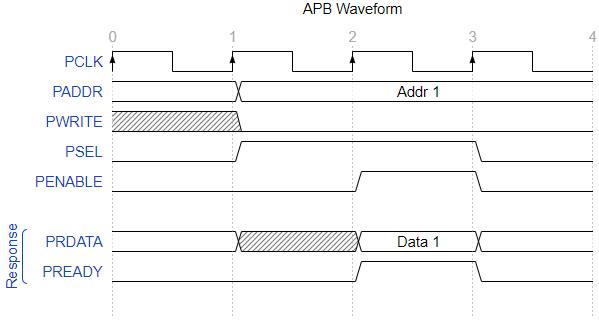
\includegraphics[width=0.7\textwidth]{apb_wave}
\caption{Waveform showing an APB read transaction.}
\end{figure}

\section{Overview}
The system-on-chip design is split into 3 main parts: peripheral interconnect (red), CPU array (gray), and the instruction memory interconnect (green).

A block diagram of this project is shown in \cref{fig:watchdog}
\begin{figure}[H]
\centering
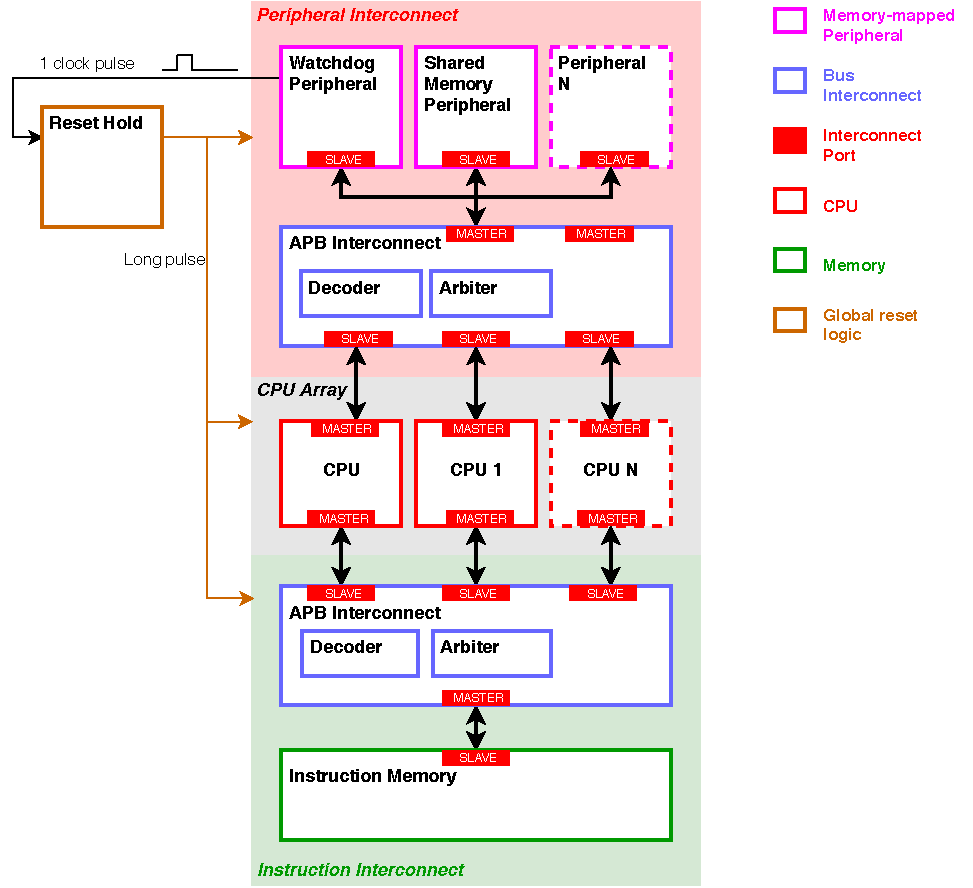
\includegraphics[width=\textwidth]{watchdog}
\caption{Block diagram of the Vmicro16 system-on-chip.}
\label{fig:watchdog}
\end{figure}

\subsection{Design Considerations}
There are several design issues to consider for this project. These are listed below:

\begin{itemize}
\item \textbf{Design size limitations}\\
The target devices for this project are small to medium sized FPGAs (featuring approximately 10,000 to 30,000 logic cells). Because of this, it is important to use a bus interconnect that has a small logic footprint yet is able to scale reasonably well.

\item \textbf{Ease of implementation}\\
The interconnect and any peripherals should be easy to implement within the time allocations specified in \cref{fig:gantt}.

\item \textbf{Scalable}\\
The interconnect should allow for easy scalability of master and slave interfaces with minimal code changes.
\end{itemize}

\section{Interfaces}

\begin{figure}[H]
\centering
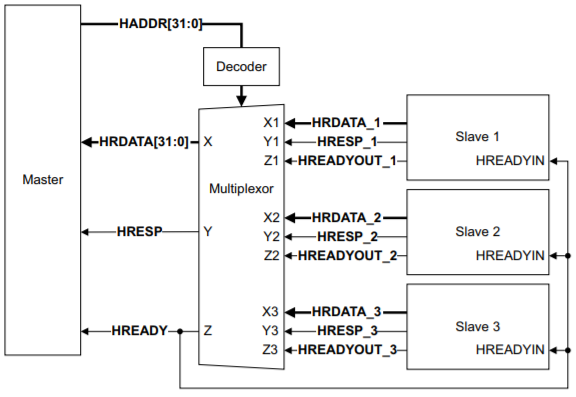
\includegraphics[width=0.7\textwidth]{ahb}
\end{figure}

\subsection{Master to Slave Interface}
\begin{figure}[H]
\centering
\begin{bytefield}[bitwidth=3.5ex, rightcurly=., rightcurlyspace=0pt]{21}
\bitheader[endianness=big]{0,15,16-20} \\
\begin{rightwordgroup}{PADDR[20:0]}
  \bitbox{1}{\rotatebox{90}{\small LE}}
  \bitbox{1}{\rotatebox{90}{\small SE}}
& \bitbox{3}{\small CORE\_ID}
& \bitbox{16}{Address}
\end{rightwordgroup}\\

\begin{rightwordgroup}{PWDATA[15:0]}
\bitbox{5}{\color{lightgray}\rule{\width}{\height}} & \bitbox{16}{Write data}
\end{rightwordgroup}\\

\begin{rightwordgroup}{PRDATA[15:0]}
\bitbox{5}{\color{lightgray}\rule{\width}{\height}} & \bitbox{16}{Read Data}
\end{rightwordgroup}\\

\begin{rightwordgroup}{PWRITE[0:0]}
\bitbox{20}{\color{lightgray}\rule{\width}{\height}} & \bitbox{1}{\rotatebox{90}{\small WE}}
\end{rightwordgroup}\\

\begin{rightwordgroup}{PENABLE[0:0]}
\bitbox{20}{\color{lightgray}\rule{\width}{\height}} & \bitbox{1}{\rotatebox{90}{\small EN}}
\end{rightwordgroup}
\end{bytefield}
\end{figure}

\newpage
\subsection{Multi-master Support}
\subsubsection{Design Goals}
\begin{enumerate}[leftmargin=3\parindent,label=\bfseries DG\arabic*.]
\item \textbf{Foo}\\
Bing
\end{enumerate}

\begin{figure}[h]
\centering
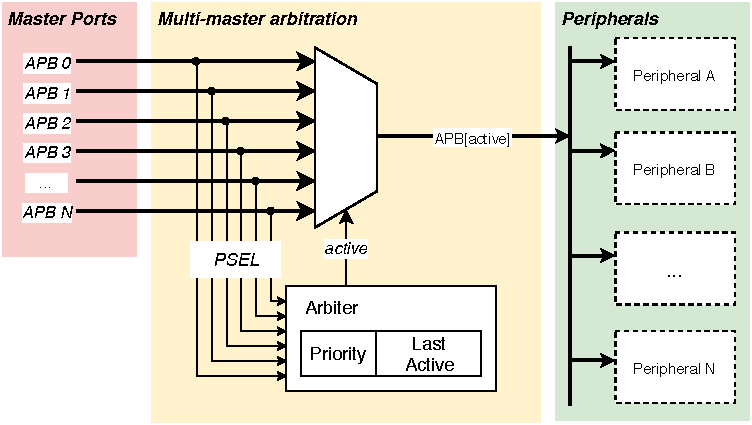
\includegraphics[width=\textwidth]{multimaster}
\caption{Foo}
\label{fig:multimaster}
\end{figure}


\begin{listing}[H]
\centering
\begin{minted}[fontsize=\footnotesize]{verilog}
input      [MASTER_PORTS*BUS_WIDTH-1:0]  S_PADDR,
input      [MASTER_PORTS-1:0]            S_PWRITE,
input      [MASTER_PORTS-1:0]            S_PSELx,
input      [MASTER_PORTS-1:0]            S_PENABLE,
input      [MASTER_PORTS*DATA_WIDTH-1:0] S_PWDATA,
output reg [MASTER_PORTS*DATA_WIDTH-1:0] S_PRDATA,
output reg [MASTER_PORTS-1:0]            S_PREADY,
\end{minted}
\caption{Variable size inputs and outputs to the interconnect.}
\end{listing}

\begin{figure}[H]
\centering
\begin{bytefield}[bitwidth=.5em, rightcurly=., rightcurlyspace=0pt]{84}
\bitheader[endianness=big]{0,20,41,62,83} \\
\bitbox{21}{Core $N$-$1$} & 
\bitbox{21}{$\cdots$} & 
\bitbox{21}{Core 1} & 
\bitbox{21}{Core 0}
\end{bytefield}
\end{figure}


\section{Further Work}
The submitted design is acceptable for a multi-core system as it fulfils the following requirements:
\begin{itemize}
\item Support an arbitrary number of peripherals.
\item Supports memory-mapped address decoding.
\item Supports multiple master interfaces.
\end{itemize}

\chapter{Memory Mapping}
{%\hypersetup{linkcolor=black}
\startcontents[chapters]
\printcontents[chapters]{}{1}{}
}
\noindent\\
The Vmicro16 processor uses a memory-mapping scheme to communicate with peripherals and other cores. This chapter describes the design decisions and implementation of the memory-map used in this project.

\section{Introduction}
Memory mapping is a common technique used by CPUs, micro-controllers, and other system-on-chip devices, that enables peripherals and other devices to be accessed via a memory address on a common bus. In a processor use-case, this allows for the reuse of existing instructions (commonly memory load/store instructions) to communicate with external peripherals with little additional logic.

\section{Address Decoding}
An address decoder is used to determine the peripheral that the address is requesting. The address decoder module, \verb|addr_dec| in \verb|apb_intercon.v|, takes the 16-bit \verb|PADDR| from the active APB interface and checks for set bits to determine which peripheral to select. The decoder outputs a chip enable signal \verb|PSEL| for the selected peripheral. For example, if bit 12 is set in \verb|PADDR| then the shared memory peripheral's \verb|PSEL| is set high and others to low. A schematic for the decoder is shown in \cref{fig:decoder}.

\begin{figure}[H]
\centering
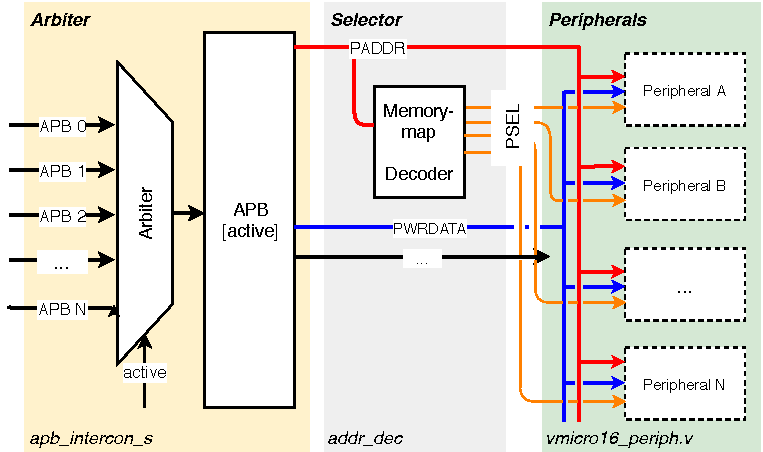
\includegraphics[width=0.8\textwidth]{decoder}
\caption{Schematic showing the address decoder (addr\_dec) accepting the active PADDR signal and outputting PSEL chip enable signals to each peripheral.}
\label{fig:decoder}
\end{figure}

\subsection{Decoder Optimisations}
Performing a 16-bit equality comparison of the \verb|PADDR| signal against each peripheral memory address consumes a significant amount of logic. Depending on the synthesis tools and FPGA features, a 16-bit comparator might require a fixed 16-bit value input to compare against (where the 0s are inverted) and a wide-AND to reduce and compare \cite{palchaudhuri2015high,salauyou2015designing}. An example 4-bit comparator is shown below in \cref{fig:comparator}.

\begin{figure}[H]
\centering
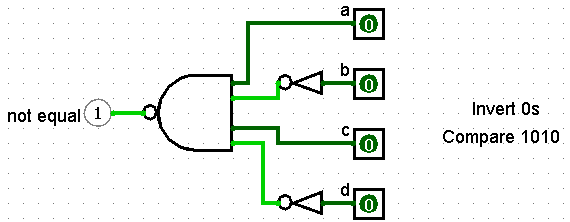
\includegraphics[width=0.5\textwidth]{comparator}
\caption{Example 4-bit binary comparator which compares the bits (a, b, c, d) to the constant value 1010. The 0s of the constant are inverted and then all are passed to a wide-AND.}
\label{fig:comparator}
\end{figure}

As we are targeting FPGAs, which use LUTs to implement combinatorial logic, we can conveniently utilise Verilog's \verb|==| operator on fairly large operands without worrying about consuming too many resources. The targeted FPGA devices in this project, the Cyclone V and Spartan 6, feature 6-input LUTs which allow 64 different configurations \cite{s6clb, cvclb}. Knowing this, we can design the address decoder to utilise the FPGA's LUTs more effectively and reduce it's footprint significantly.

We can use part of the \verb|PADDR| signal as a chip select and the other bits as sub-addresses to interface with the peripheral. The addressing bits are passed into the FPGA's 6-input LUTs which are programmed (via the bitstream) to output 1 or 0 depending on the address. \cref{fig:comparatorlut} below shows a LUT based approach to address decoding which will utilise approximately one ALM/CLB module per peripheral chip select (\verb|PSEL|) and one for error detection. This method of comparison (LUT based) is utilised in the \verb|addr_dec| module in \verb|apb_intercon.v|.

\begin{figure}[H]
\centering
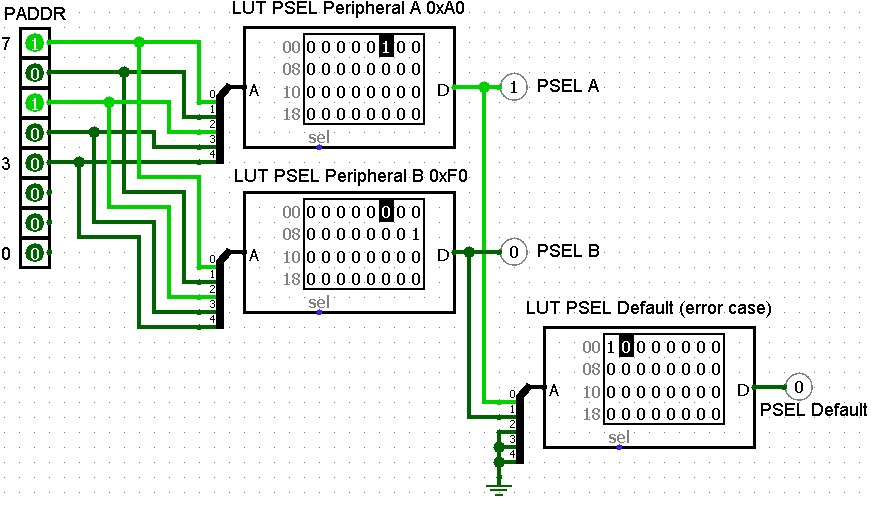
\includegraphics[width=0.8\textwidth]{comparatorlut}
\caption{Bits [7:3] of an 8-bit PADDR signal are used as inputs to 5-bit LUTs to generate a PSEL signal. In addition, a default error case is shown allowing the address decoder to detect incorrect PADDR values (e.g. if no PSEL signals are generated).}
\label{fig:comparatorlut}
\end{figure}

The address decoding methods discussed above are examples of \textit{full-address} decoding, where each bit (whether required or not) is compared. It is possible to further reduce the required logic by utilising \textit{partial-address} decoding \cite{tanenbaum2016structured}. Partial-address decoding can reduce logic requirements by not using all bits. For example, if bits in address \verb|0x0100| do not conflict with bits in other addresses (i.e. bit 8 is high in more than 1 address), then the address decoder needs only concern bit 8, not the other bits. This is visualised in \cref{fig:partial} below. This method is utilised in the MMU's address decoder (module \verb|vmicro16_mmu| in \verb|vmicro16.v:181|). As this is an optimisation per core, significant resources can be saved when a large number of cores are used.

\begin{figure}[H]
\centering
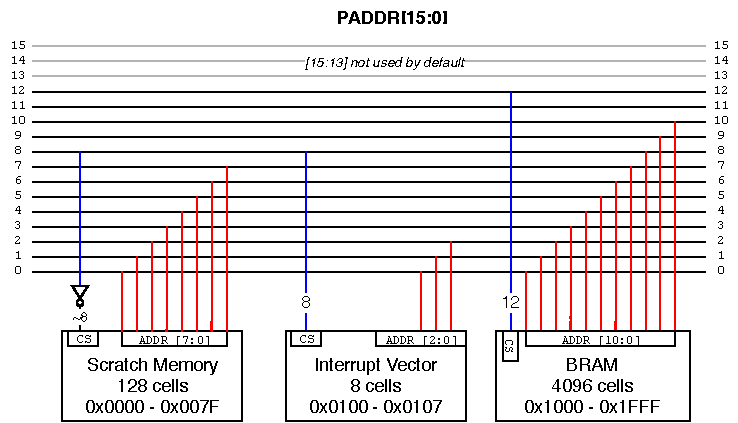
\includegraphics[width=0.8\textwidth]{partial}
\caption{Partial address decoding used by the Vmicro16 SoC design. Each peripheral shown only needs to decode a signal bit to determine if it is enabled.}
\label{fig:partial}
\end{figure}

\section{Memory Map}
The system-on-chip's memory map is shown below in \cref{fig:memmap}. The addresses for each peripheral have been carefully chosen for both:
\begin{itemize}
\item Easy software access -- creating addresses via software requires few instructions (normally one to four \verb|MOVI| and \verb|LSHIFT| instructions to address \verb|0x0000| to  \verb|0xffff|), which increases software performance.
\item and Reducing address decoding logic -- most addresses can be decoded using partial decoding techniques.
\end{itemize}

\begin{figure}[H]
\centering
\begin{bytefield}{24}
	\memsection{1FFF}{1000}{8}{Shared Memory with Global Monitor \\ \vspace{.5cm} \tiny See vmicro16\_soc\_config.v}\\
	\bitbox[]{16}{} & \bitbox[]{16}{$\vdots$ \\[1ex]} \\
	
	\begin{rightwordgroup}{Shared peripherals}
	\memsection{0202}{0200}{3}{\nameref{sect:timer}}
	\end{rightwordgroup}\\
	\bitbox[]{16}{} & \bitbox[]{16}{$\vdots$ \\[1ex]} \\
	
	\begin{rightwordgroup}{Per-core instances}
	\memsection{0108}{}{1}{\nameref{sect:interrupts} Mask}\\
	\memsection{0107}{0100}{3}{\nameref{sect:interrupts} Vector}
	\end{rightwordgroup}\\
	
	\bitbox[]{16}{} & \bitbox[]{16}{$\vdots$ \\[1ex]} \\
	
	\begin{rightwordgroup}{Shared peripherals}
	\memsection{00B8}{}{1}{\nameref{sect:watchdog}}\\
	\memsection{00B7}{00B0}{3}{REGS0}\\
	\bitbox[]{16}{} & \bitbox[]{16}{$\vdots$ \\[1ex]} \\
	\memsection{00A1}{00A0}{2}{UART0}\\
	\bitbox[]{16}{} & \bitbox[]{16}{$\vdots$ \\[1ex]} \\
	\memsection{0092}{}{1}{GPIO2}\\
	\memsection{0091}{}{1}{GPIO1}\\
	\memsection{0090}{}{1}{GPIO0}
	\end{rightwordgroup}\\
	\bitbox[]{16}{} & \bitbox[]{16}{$\vdots$ \\[1ex]} \\
	
	\begin{rightwordgroup}{Per-core instances}
	\memsection{008F}{0080}{3}{16 Special Registers}\\
	\memsection{007F}{0000}{8}{Scratch Memory \\ \vspace{.5cm} \tiny See vmicro16\_soc\_config.v}
	\end{rightwordgroup}\\
	
\end{bytefield}
\caption{Memory map showing addresses of various memory sections.}
\label{fig:memmap}
\end{figure}

